\documentclass{article}
% Change page layout
\usepackage[margin=2cm]{geometry}
\usepackage{xcolor}
\usepackage{tensor}
\usepackage{parskip}
\usepackage{amsmath, amssymb}
\usepackage{gensymb}
\usepackage{cancel}
\usepackage{hyperref}

\hypersetup{
    colorlinks=true,
    urlcolor=blue
}

\usepackage{pgfplots}
\pgfplotsset{compat=1.18}

\let\vec\mathbf

\begin{document}
\newcommand{\assignmenttitle}[2]{
    \begin{flushleft}
        \begin{Huge}
            #1
        \end{Huge}
    \end{flushleft}
    \vspace{-0.8em}
    \hrulefill

    \vspace{-0.8em}
    #2 \hfill Mainak Roy 

    \vspace{-1.4em}
    \hrulefill
}
\assignmenttitle{Classical Electrodynamics II}{Assignment 1}

\emph{Code link:} \url{https://github.com/Newtech66/TIFR-ED2} 

\section*{P1}
\emph{(skipped)}
\section*{P2}
\subsection*{(a)}
The Lorentz transformation is given by
\begin{align}
    ct' &= \gamma\left(ct-\frac{vx}{c}\right)\\
    x' &= \gamma\left(x-\frac{v}{c}ct\right)
\end{align}
We can treat $ct$ and $x$ as unit vectors and then calculate the angle between $ct'$ and $x'$.
\begin{equation}
    \cos\theta = \frac{ct'\cdot x'}{|ct'||x'|} = \frac{-\frac{2v}{c}}{1+\frac{v^2}{c^2}}
\end{equation}
\begin{figure}[h]
    \centering
    \begin{tikzpicture}
        \begin{axis}[
            xmin=0,xmax=1,
            samples=1000,
            grid=both,
            ymin=90,ymax=180,
            xlabel=$v$,
            ylabel=$\theta$,
            xticklabels={,0,0.2$c$,0.4$c$,0.6$c$,0.8$c$,$c$},
            yticklabel={$\pgfmathprintnumber{\tick}^{\degree}$},
            ytick distance=15
            ]
            \addplot[raw gnuplot, color=red] gnuplot [id=axes_orth]{
                set angle degrees;
                set xrange[0:1];
                plot acos(-2*x/(1+x^2));
            };
        \end{axis}
    \end{tikzpicture}
    \caption{Variation of angle between $ct$ and $x$ as a function of velocity.}
\end{figure}
\begin{figure}[h]
    \centering
    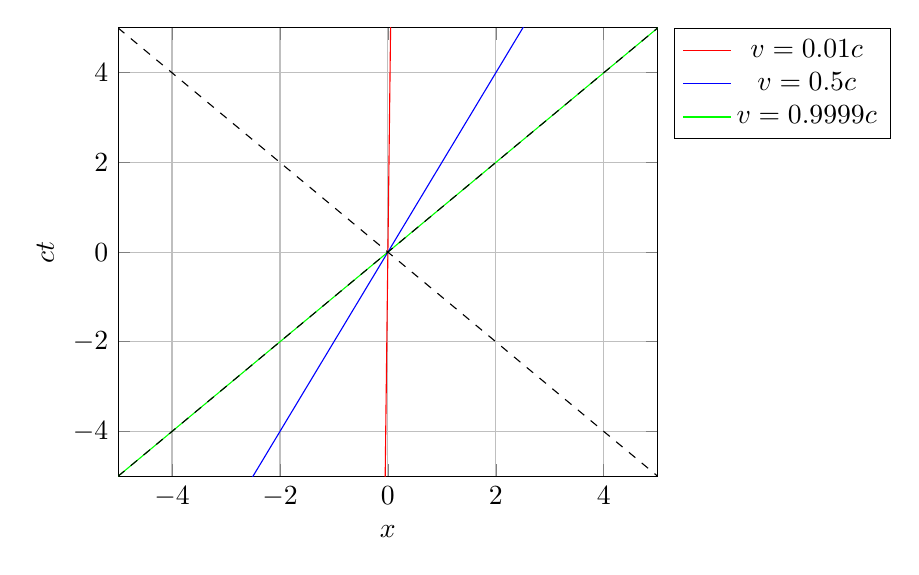
\begin{tikzpicture}
        \begin{axis}[
            xlabel=$x$,
            ylabel=$ct$,
            grid=both,
            xmin=-5,xmax=5,
            ymin=-5,ymax=5,
            legend entries={$v=0.01c$,$v=0.5c$,$v=0.9999c$},
            legend pos=outer north east
        ]
            \addplot[color=red]{(1/0.01)*x};
            \addplot[color=blue]{(1/0.5)*x};
            \addplot[color=green]{(1/0.9999)*x};
            \addplot[dashed]{x};
            \addplot[dashed]{-x};
        \end{axis}
    \end{tikzpicture}
    \caption{Space-time diagram for objects travelling at different velocities.}
\end{figure}

\subsection*{(b)}
Say the object sends a light signal towards us at $t=0$ while it is at a distance $d$ from us. The light signal arrives to us at time $t_1=d/c$. Now let a small time $\Delta t$ pass, and then another light signal is sent towards us from the new position. The signal arrives to us at time
\begin{align}
    t_2 &= \Delta t + \frac{\sqrt{(v_s\Delta t\sin\alpha)^2+(d-v_s\Delta t\cos\alpha)^2}}{c}\\
    &= \Delta t + \frac{\sqrt{\cancel{(v_s\Delta t)^2}+d^2-2dv_s\Delta t\cos\alpha}}{c}\\
    &\approx \Delta t + \frac{d}{c}\left(1-\frac{v_s\Delta t\cos\alpha}{d}\right)
\end{align}
The apparent transverse speed of the object is given by
\begin{align}
    v &= \frac{v_s\Delta t\sin\alpha}{t_2 - t_1}\\
    &= \frac{v_s\Delta t\sin\alpha}{\Delta t\left(1-\frac{v_s\cos\alpha}{c}\right)}
\end{align}
\begin{equation}
    \boxed{v = \frac{v_s\sin\alpha}{1- \frac{v_s\cos\alpha}{c}}}
\end{equation}

\section*{P3}
We know the lifetime of the particle in its rest frame is constant. But if we Lorentz transform to the lab frame, because of time dilation it appears to us that the particle's lifetime is longer.
\begin{equation}
    t = \frac{\tau}{\sqrt{1-\frac{v^2}{c^2}}}
\end{equation}
\begin{figure}[h]
    \centering
    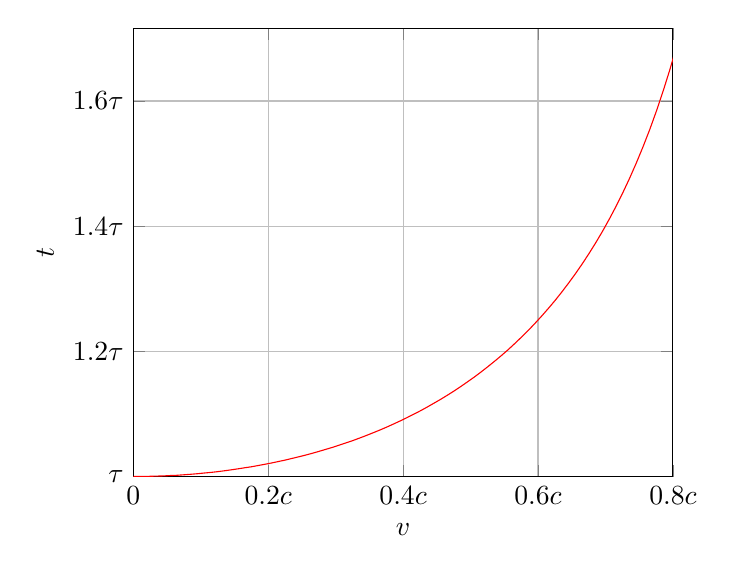
\begin{tikzpicture}
        \begin{axis}[
            xmin=0,xmax=0.8,
            samples=1000,
            grid=both,
            ymin=1,
            xlabel=$v$,
            ylabel=$t$,
            xticklabels={,0,0.2$c$,0.4$c$,0.6$c$,0.8$c$},
            yticklabels={,$\tau$,1.2$\tau$,1.4$\tau$,1.6$\tau$},
            ]
            \addplot[color=red]{1/sqrt(1-x^2)};
        \end{axis}
    \end{tikzpicture}
    \caption{Variation of lifetime of particle in lab frame.}
\end{figure}
\begingroup
\renewcommand{\labelenumi}{\theenumi}
\renewcommand{\theenumi}{(\roman{enumi})}
\begin{enumerate}
    \item $t=1.00005\tau$
    \item $t=1.1547\tau$
    \item $t=70.7124\tau$
\end{enumerate}
\endgroup
\section*{P4}
\emph{(skipped)}
\section*{P5}
The electromagnetic field tensor is given by
\begin{equation}
    F^{ik}=\begin{pmatrix}
        0 & -E_x & -E_y & -E_z \\
        E_x & 0 & -B_z & B_y \\
        E_y & B_z & 0 & -B_x \\
        E_z & -B_y & B_x & 0
    \end{pmatrix}
\end{equation}
The relativistic force equation is given by
\begin{equation}
    mc\frac{du^i}{ds}=\frac{q}{c}F^{ik}u_k
\end{equation}
The relation between $ds$ and $dt$ is given by
\begin{gather}
    \gamma=\frac{1}{\sqrt{1-\frac{v^2}{c^2}}}\\
    ds = \frac{cdt}{\gamma}
\end{gather}
The relation between 4-velocity is given by
\begin{gather}
    x^i=(ct,\vec{x})\\
    \frac{dx^i}{dt}=(c,\vec{v})\\
    u^i = \frac{dx^i}{ds} = \frac{dt}{ds}\frac{dx^i}{dt}
\end{gather}
We can compute the spatial part
\begin{gather}
    mc^2\frac{d}{dt}\left(\frac{dx^\alpha}{ds}\right) = qF^{\alpha k}\frac{dx_k}{dt}\\
    mc^2\frac{d}{dt}\left(\frac{dt}{ds}\vec{v}\right)=q
    \begin{pmatrix}
        cE_x + v_yB_z - v_zB_y\\
        cE_y -v_xB_z + v_zB_x\\
        cE_z + v_xB_y - v_yB_x
    \end{pmatrix} = qc\vec{E} +q\vec{v}\times\vec{B}\\
    mc\vec{v}\frac{d\gamma}{dt}+mc\gamma\frac{d\vec{v}}{dt}=qc\vec{E}+q\vec{v}\times\vec{B}
\end{gather}
We can compute the time part
\begin{gather}
    mc^2\frac{d}{dt}\left(\frac{dx^0}{ds}\right) = qF^{0 k}\frac{dx_k}{dt}\\
    mc\frac{d\gamma}{dt} = \frac{q}{c}\vec{v}\cdot \vec{E}
\end{gather}
Therefore
\begin{equation}
    \frac{d\vec{v}}{dt}=\frac{q}{m}\sqrt{1-\frac{v^2}{c^2}}\left(\vec{E}+\frac{1}{c}\vec{v}\times\vec{B} - \frac{1}{c^2}\vec{v}(\vec{v}\cdot \vec{E})\right)
\end{equation}

\section*{P6}
\subsection*{(a)}
We can do this by Lorentz boosting the electromagnetic field tensor. Let the linear charge density be $\lambda$. In the rest frame, the electric field can be found in cylindrical coordinates with Gauss' law as
\begin{equation}
    \vec{E} = \frac{\lambda}{2\pi\rho\epsilon_0}\hat{\rho}
\end{equation}
So, the electromagnetic field tensor in the rest frame is given by
\begin{equation}
    F^{ik} = \frac{\lambda}{2\pi\epsilon_0}\begin{pmatrix}
        0 & \frac{-x}{x^2+y^2} & \frac{-y}{x^2+y^2} & 0\\
        \frac{x}{x^2+y^2} & 0 & 0 & 0 \\
        \frac{y}{x^2+y^2} & 0 & 0 & 0 \\
        0 & 0 & 0 & 0
    \end{pmatrix}
\end{equation}
The Lorentz transformation matrix for a boost along the length of the line charge is given by
\begin{gather}
    \gamma=\frac{1}{\sqrt{1-\frac{v^2}{c^2}}}\\
    \Lambda\indices{^i_k}=\begin{pmatrix}
        \gamma & 0 & 0 & -\gamma \frac{v}{c}\\
        0 & 1 & 0 & 0\\
        0 & 0 & 1 & 0\\
        -\gamma \frac{v}{c} & 0 & 0 & \gamma
    \end{pmatrix}
\end{gather}
The Lorentz boosted electromagnetic field tensor is
\begin{align}
    F^{ab} &= \Lambda\indices{^a_c}\Lambda\indices{^b_d}F^{cd}\\
    &=\frac{\gamma\lambda}{2\pi\epsilon_0}
\begin{pmatrix}
    0 & \frac{-x}{x^2+y^2} & \frac{-y}{x^2+y^2} & 0\\
    \frac{x}{x^2+y^2} & 0 & 0 & \frac{-x}{x^2+y^2}\frac{v}{c} \\
    \frac{y}{x^2+y^2} & 0 & 0 & \frac{-y}{x^2+y^2}\frac{v}{c} \\
    0 & \frac{x}{x^2+y^2}\frac{v}{c}  & \frac{y}{x^2+y^2}\frac{v}{c} & 0
\end{pmatrix}
\end{align}
which simplifies in cylindrical coordinates to
\begin{align}
    \vec{E} &= \frac{\gamma\lambda}{2\pi\rho\epsilon_0}\hat{\rho}\\
    \vec{B} &= -\frac{\gamma\lambda}{2\pi\rho\epsilon_0}\frac{v}{c}\hat{\varphi}
\end{align}

\subsection*{(b)}
We have that
\begin{gather}
    \partial_{i}F^{ik}=\frac{1}{c}J^{k}\\
    J^{k}=(c\rho, \vec{j})
\end{gather}
We can compute
\begin{equation}
    \partial_{i}J^{i} = \partial_{i}\partial_{j}F^{ji} = 0
\end{equation}
Therefore,
\begin{equation}
    \frac{\partial\rho}{\partial t} + \nabla \cdot \vec{j} = 0
\end{equation}
which is the continuity equation.

\section*{P7}
\subsection*{(a)}
The first pair of Maxwell equations are given by
\begin{equation}
    \partial_{i}F^{ik} = \frac{1}{c}J^{k}
\end{equation}
We can expand it to
\begin{equation}
    \begin{pmatrix}
        \nabla \cdot \vec{E} \\
        (\nabla \times \vec{B})_{x}-\frac{1}{c}\frac{\partial E_{x}}{\partial t}\\
        (\nabla \times \vec{B})_{y}-\frac{1}{c}\frac{\partial E_{y}}{\partial t}\\
        (\nabla \times \vec{B})_{z}-\frac{1}{c}\frac{\partial E_{z}}{\partial t}
    \end{pmatrix}
    =
    \frac{1}{c}
    \begin{pmatrix}
        c\rho\\
        j_x\\
        j_y\\
        j_z
    \end{pmatrix}
\end{equation}
which reduces to
\begin{gather}
    \nabla \cdot \vec{E} = \rho\\
    \nabla \times \vec{B} = \frac{1}{c}\left(\frac{\partial E}{\partial t} + \vec{j}\right)
\end{gather}

The second pair of Maxwell equations are given by
\begin{equation}
    \partial_{i}\left(\varepsilon\indices{^{ijkl}}F_{kl}\right) = 0
\end{equation}

We can find that
\begin{equation}
    \frac{1}{2}\varepsilon\indices{^{ijkl}}F_{kl} = 
    \begin{pmatrix}
        0 & -B_x & -B_y & -B_z \\
        B_x & 0 & E_z & -E_y \\
        B_y & -E_z & 0 & E_x \\
        B_z & E_y & -E_x & 0
    \end{pmatrix}
\end{equation}
and then we can find that
\begin{equation}
    \begin{pmatrix}
        \nabla \cdot \vec{B} \\
        -(\nabla \times \vec{E})_{x}-\frac{1}{c}\frac{\partial B_{x}}{\partial t}\\
        -(\nabla \times \vec{E})_{y}-\frac{1}{c}\frac{\partial B_{y}}{\partial t}\\
        -(\nabla \times \vec{E})_{z}-\frac{1}{c}\frac{\partial B_{z}}{\partial t}
    \end{pmatrix} = 0
\end{equation}
which reduces to
\begin{gather}
    \nabla \cdot \vec{B} = 0 \\
    \nabla \times \vec{E} = -\frac{1}{c}\frac{\partial \vec{B}}{\partial t}
\end{gather}

\subsection*{(b)}
We can expand
\begin{align}
    \tilde{F}^{lm}F_{lm} &= \varepsilon\indices{^{iklm}}F_{ik}F_{lm}\\
    &= \varepsilon\indices{^{iklm}} (\partial_i A_k - \partial_k A_i) (\partial_l A_m - \partial_m A_l)\\
    &=\varepsilon\indices{^{iklm}}\partial_i A_k \partial_l A_m\\
    &-\varepsilon\indices{^{iklm}}\partial_i A_k \partial_m A_l\\
    &-\varepsilon\indices{^{iklm}}\partial_k A_i \partial_l A_m\\
    &+\varepsilon\indices{^{iklm}}\partial_k A_i \partial_m A_l\\
\end{align}

We can use the antisymmetry of $\varepsilon\indices{^{iklm}}$ to rearrange the indices. So we get
\begin{equation}
    \tilde{F}^{lm}F_{lm} = 4\partial_i (\varepsilon\indices{^{iklm}}A_k \partial_l A_m)
\end{equation}
This is a 4-divergence, which does not affect the action. So it has no effect on the equations of motion.

\hrulefill
\end{document}